% 精确坐标：共焦点 F1=(-2,0), F2=(2,0)
% 椭圆 E: x^2/16 + y^2/12 = 1 (e1=1/2)
% 双曲线 H: x^2 - y^2/3 = 1 (e2=2)
% P=(2,3), PF1=5, PF2=3, F1F2=4, cos(theta)=3/5
% 所有几何点与图形由真实方程指定，并非自由手绘。
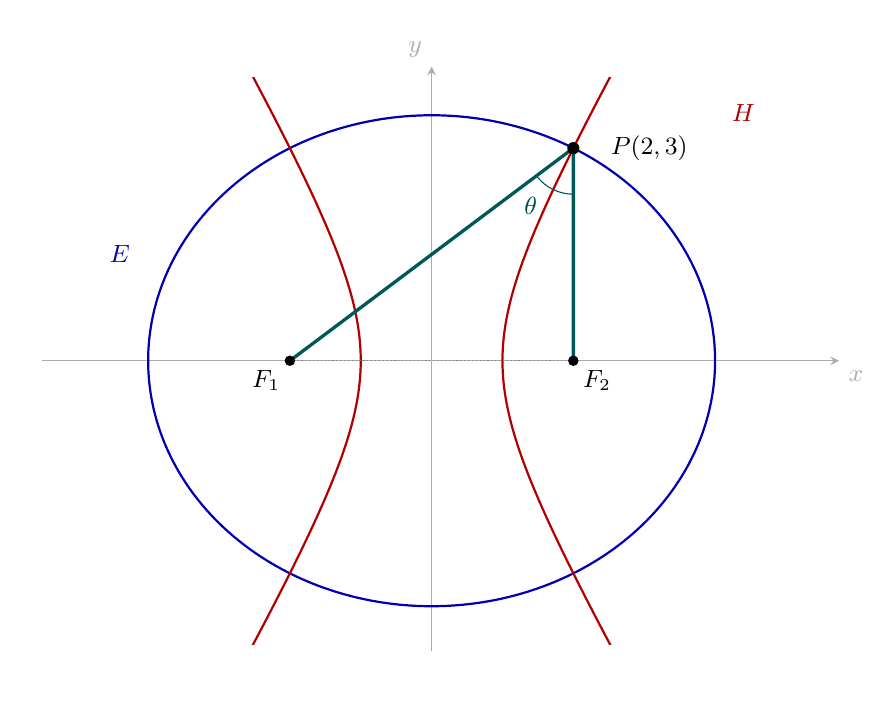
\begin{tikzpicture}[x=0.9cm,y=0.9cm,>=stealth,every node/.style={font=\small}]
  \path[use as bounding box] (-5.7,-4.5) rectangle (6.0,4.7);
  \draw[->,gray!65,thin] (-5.5,0)--(5.75,0) node[below right] {$x$};
  \draw[->,gray!65,thin] (0,-4.1)--(0,4.15) node[above left] {$y$};
  \begin{scope}
  \clip (-5.2,-4) rectangle (5.2,4);
  \draw[thick,blue!70!black,domain=0:360,samples=181,smooth,variable=\t]
    plot ({4*cos(\t)},{sqrt(12)*sin(\t)});
  \draw[thick,red!70!black,domain=-70:70,samples=131,smooth,variable=\t]
    plot ({1/cos(\t)},{sqrt(3)*tan(\t)});
  \draw[thick,red!70!black,domain=-70:70,samples=131,smooth,variable=\t]
    plot ({-1/cos(\t)},{sqrt(3)*tan(\t)});
  \end{scope}
  \coordinate (Fone) at (-2,0);
  \coordinate (Ftwo) at (2,0);
  \coordinate (PP) at (2,3);
  \draw[very thick,teal!70!black] (PP)--(Fone) (PP)--(Ftwo);
  \draw[thin,densely dotted,gray] (Fone)--(Ftwo);
  \fill[black] (Fone) circle(1.9pt) node[below left] {$F_1$};
  \fill[black] (Ftwo) circle(1.9pt) node[below right] {$F_2$};
  \fill[black] (PP) circle(2.2pt) node[right,xshift=10pt] {$P(2,3)$};
  \draw[teal!70!black] (2,2.35) arc[start angle=-90,end angle=-143.130102,radius=0.65];
  \node[teal!60!black] at (1.40,2.18) {$\theta$};
  \node[blue!70!black] at (-4.4,1.5) {$E$};
  \node[red!70!black] at (4.4,3.5) {$H$};
\end{tikzpicture}
